\scanpage{26}\mspage{20}
% @ top, continuation | text | en épinglant le triangle
en épinglant le triangle $u,v,w$ i.e. l'arête $(v,w)$ par choix d'une ``origine'' $v$ -- i.e. partant d'un \uline{arc} \inserted{$\vec\alpha$} plutôt que d'une arête $\alpha$. \deleted{Alors}, Cel\unsure{a} signifie aussi (comme $\{v,w\}=P\wedge_{\mathbb F_2^{P_u}}(\mathbb F_2,\varepsilon)$) qu'on a restreint le groupe structural de $\mathbb F_2^{P_u}$ : $\Psi_{P_u}=\operatorname{Ker}(\mathbb F_2^{P_u}\overset{\varepsilon}{\longrightarrow}\mathbb F_2)$. On trouve donc l'extension splittée
% @ top third, extension | diagram | 1, Ψ, W, symmetric group, 1
\diagram{\begin{tikzcd}[ampersand replacement=\&,column sep=large]
1\arrow[r,dash]\&\Psi_{P_u}\arrow[r,dash]\&W_{\vec\alpha}\inserted{=W_t}\arrow[r,dash]\&\unsure{\mathfrak S|\mathscr S}_{P_u}\arrow[r,dash]\&1
\end{tikzcd}}
% @ upper middle, identification | text | donc
donc
% @ upper middle, W | display | W of the directed edge
\[
W_{\vec\alpha}\simeq W_{D_4}
\]
\margin{autom de $C$ qui sont l'identité sur $t=\{u,v,w\}$}

% @ middle, root count | text | groupe de Weyl de D₄
groupe de Weyl de $D_4$ $(\simeq\mathrm{so}(8))$. Ce syst. de racines (ttes de $=$ longueur) à $\frac{8.7}{2}-4=24$ racines. On retrouve $W_t$ par une description plus symétrique (en $u,v,w$) plus bas, ainsi qu'une description plausible du syst de 24 racines de type $D_4$ associé à un triangle \ldots.

% @ right margin, drawings and words | text | Complexe cubique avec balai
\margin{Complexe cubique avec balise \unsure{marquée|marqué} ou à \inserted{couple de} triangles incidents marqué}
% @ right, beside first phrase | diagram | v w above u ; lower end a
\diagram{\begin{tikzcd}[ampersand replacement=\&,execute at end picture={
\draw[thick](0,1)node[above left]{$v$}--(.6,1)node[above right]{$w$}--(.29,.53)node[left]{$u$}--cycle;
\draw[thick](.29,.53)--(.31,-.13)node[below right]{$a$};}]\vphantom{A}\end{tikzcd}}
% @ right, beside second phrase | diagram | v w, u, a b
\diagram{\begin{tikzcd}[ampersand replacement=\&,execute at end picture={
\draw(0,1)node[above left]{$v$}--(.65,1)node[above right]{$w$}--(.31,.49)node[left]{$u$}--cycle;
\draw(.31,.49)--(.04,-.12)node[below left]{$a$}--(.65,-.12)node[below right]{$b$}--cycle;
\fill(.31,.49) circle (1.4pt);}]\vphantom{A}\end{tikzcd}}
% @ centre below paragraph, divider | drawing | two horizontal strokes joined by a loop
\figure{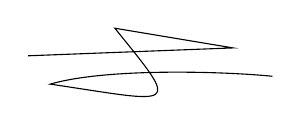
\begin{tikzpicture}\draw(0,0)--(2.6,.1)--(1.1,.35)..controls(1.95,-.7) and (1.9,-.6)..(.28,-.36)..controls(1,-.15) and (2.5,-.2)..(3.1,-.26);\end{tikzpicture}}

% @ lower third, heading | text | Complexe cubique à triangle marqué
\uline{Complexe cubique à triangle \inserted{$t$} marqué}, $t=\{u,v,w\}$.

% @ lower third, opening | text | Équivaut à la donnée
Équivaut à la donnée

% @ foot, a | text | d'un t
a) d'un \deleted{\unsure{ens.}} $t$ de cardinal 3

% @ foot, b | text | d'un vectoriel
b) d'un vectoriel $N$ de dim 2 sur $\mathbb F_2$ ($\Longleftrightarrow$ ens de cardinal 3 savoir $V^*$)

% @ foot, c | text | Un torseur
c) Un torseur $\widetilde P$ sous l'extension canonique
% archive sheet number: 25
